% TEMPLATE for Usenix papers, specifically to meet requirements of
%  USENIX '05
% originally a template for producing IEEE-format articles using LaTeX.
%   written by Matthew Ward, CS Department, Worcester Polytechnic Institute.
% adapted by David Beazley for his excellent SWIG paper in Proceedings,
%   Tcl 96
% turned into a smartass generic template by De Clarke, with thanks to
%   both the above pioneers
% use at your own risk.  Complaints to /dev/null.
% make it two column with no page numbering, default is 10 point

% Munged by Fred Douglis <douglis@research.att.com> 10/97 to separate
% the .sty file from the LaTeX source template, so that people can
% more easily include the .sty file into an existing document.  Also
% changed to more closely follow the style guidelines as represented
% by the Word sample file. 

% Note that since 2010, USENIX does not require endnotes. If you want
% foot of page notes, don't include the endnotes package in the 
% usepackage command, below.

% This version uses the latex2e styles, not the very ancient 2.09 stuff.
%\documentclass[letterpaper,twocolumn,10pt]{article}
\documentclass[10pt,reprint]{socc14}

\special{papersize=8.5in,11in}
\setlength{\pdfpageheight}{\paperheight}
\setlength{\pdfpagewidth}{\paperwidth}

\conferenceinfo{Research Proficiency Exam Report}{August, 2014, Stony Brook, NY, USA} 
\copyrightyear{2014} 
\copyrightdata{978-1-nnnn-nnnn-n/yy/mm} 
\doi{nnnnnnn.nnnnnnn}

%\usepackage{usenix,epsfig,endnotes}
\usepackage{epsfig,endnotes}
\usepackage[english]{babel}
\usepackage{color}
\usepackage{needspace}
\usepackage{amsfonts}
\usepackage{amsmath, amssymb}
\usepackage{epsfig}
\usepackage{url}
\usepackage{tabularx}
\usepackage{todonotes}
\usepackage{algorithm, algorithmic}
\usepackage{wrapfig}
\usepackage{multirow}
\usepackage{graphicx, subfigure}
\usepackage{booktabs}
\usepackage{dcolumn}
\usepackage{array}
\usepackage{listings}
\newcommand{\dpi}[1]{{\textcolor{red}{\bf #1}}}
\setlength{\marginparwidth}{2cm}
% \def\todo#1{\textbf{[TODO:~#1]}\footnote{TODO:~#1}}
\def\todox#1{{\bf \textcolor{red}{TODO:~#1}}}
\def\etal{et\ al.\ }

%\def\sysname{DIMMer~}

\begin{document}

%don't want date printed
\date{}

%make title bold and 14 pt font (Latex default is non-bold, 16 pt)
\title{Secure Execution of Mutually Mistrusting Software}
\subtitle{}
%{Turn Off Memory and CPU: a Great Fertilizer for Green Data Centers!}

%for single author (just remove % characters)

\authorinfo{Dongli Zhang}
           {Stony Brook University}
		   {dozhang@cs.stonybrook.edu}

\maketitle
%
%% Use the following at camera-ready time to suppress page numbers.
%% Comment it out when you first submit the paper for review.
%\thispagestyle{empty}
%

\subsection*{Abstract}
Commodity operating systems, e.g. Linux and Android, running on PC or
smartphone, are ubiquitous in home, commercial, government, and military
settings. The booming popularity of PC and smartphone makes the commodity
operating system an attractive target for attacks. These systems are tasked with
a variety of applications, e.g. from secure software provided by trusted
organizations to regular applications including games and web browsers
downloaded from untrusted third-party website.

Since PC and smartphone are used both for working and entertainment, both
trusted and untrusted applications are installed on the commodity operating
system. The complex interface between malicious applications and the operating
system kernel makes the latter one vulnerable to malwares. The compromised
untrusted operating system is able to break both privacy and integrity of secure
applications. The user mode secure application is not tamper-resistant to the
privileged operating system kernel.

Various methods have been proposed to execute mutually mistrusting software on
commodity operating systems. In this talk, we divide the state of the art
research papers into three classes. First, we discuss how to protect the secure
application from the untrusted operating system. Second, we discuss the
isolation of untrusted application from the benign operating system. Third, we
discuss how to remove the trust relationship between application and operating
system, that is, neither application nor operating system trust each other. We
finally propose an framework for the secure execution of sensitive code on ARM
architecture.
%\end{abstract}

\section{Introduction}
\label{sec:introduction}

Nowadays, PC and smartphone running the commodity operating systems, which are
ubiquitous in home, commercial, government and military settings, become
significantly indispensable in our life. According to a report from Gartner
\cite{Gartner}, the
worldwide PC shipments totaled 82.6 million units just in the fourth quarter of
2013.  The most popular operating systems on PC are Windows, Linux and Mac OS
and various applications are installed and executed on the commodity operating
system every day. Besides PC, recent years have also experienced explosive
growth of smartphone sales. Inevitably, the rise in the popularity of
smartphones also makes them an attractive target for attacks. According to the
report from Canalys \cite{Canalys}, the year of 2011 marks as the first time in history that
smartphones have outsold PCs. Their booming popularity can be partially
attributed to their improved functionality and convenience for end users. 

PCs are used for a variety of daily works such as checking emails, video
conference and data processing. Smartphones are also no longer basic devices for
making phone calls and receiving text messages, but powerful platforms, with
comparable computing and communication capabilities to commodity PCs, for video
conference, gaming, and even online shopping. Generally, different applications
have disparate level of security requirement. For instance, on a smartphone
running Android, the online banking application has a higher level of security
than the Angry Birds.

The execution of mutually mistrusting software brings security trouble to the
commodity operating systems. Suppose the PC is running a Linux operating system.
The user might use the PC to view a lot of PDF files every day. The PDF file
injected with malware is able to infect the operating system because of the
complex interface between the application and the operating system. Latter, the
user may login into the online bank account to check the deposit. As the
underpinning privileged operating system, including keyboard driver, has already
been compromised, the browser’s privacy, i.e. the user’s credentials, will be
stolen by the attacker.

Another example is on a smartphone running an Android operating system. Users
are suggested to download Android applications from official website, such as
Google Online Store. However, many users download repacked applications, e.g.
games, from the third-part website. For instance, without protection, the
malicious repacked gaming application is able to elevate the privilege and
compromise the Android runtime and even the Linux kernel. The compromised
Android operating system is able to defect the privacy and integrity of other
applications, e.g. the user’s identification of Facebook.

In this talk, we discuss the solutions for the problems introduced by the
execution of mutually mistrusting software. We formulate the problems into three
sub-problems. The first problem is to protect the secure application or
sensitive PAL (Pieces of Application Logic) from the untrusted operating system.
Commodity operating systems entrusted with securing sensitive data are
remarkably large and complex, and consequently, frequently prone to compromise.
The privacy and integrity of the application are expected to be protected even
in the event of a total OS compromise. Solutions to this problem has a variety
of applications in real life from protecting the privacy and integrity
certificate generation on a CA server to isolating the sensitive list of
Transaction Authentication Numbers (TAN) from the untrusted Android operating
system on a smartphone.

The second problem is to isolate the untrusted application or a piece of code
from the operating system. Modern commodity operating systems are underpinning
many applications from different sources. The complex interface between the
application and the operating system opens a large attack surface for the
misbehaving application to compromise the rest of the operating system. The
operating system can be compromised by a piece of native code downloaded and
executed by the web browser with mechanisms such as ActiveX and NPAPI or an
Android application infected by DKFBootKit \cite{DKFBootKit}.

The third problem is how to establish the two-way protection, that is, to
protect the application from the operating system while to protect the operating
system from the application. We rethink the security model and argue that a
two-way sandbox is desired.  We discuss MiniBox \cite{MiniBox}, the first paper
aiming at removing the trust between applications and the operating system of
PaaS cloud computing.

\begin{figure*}[htb]
\centering
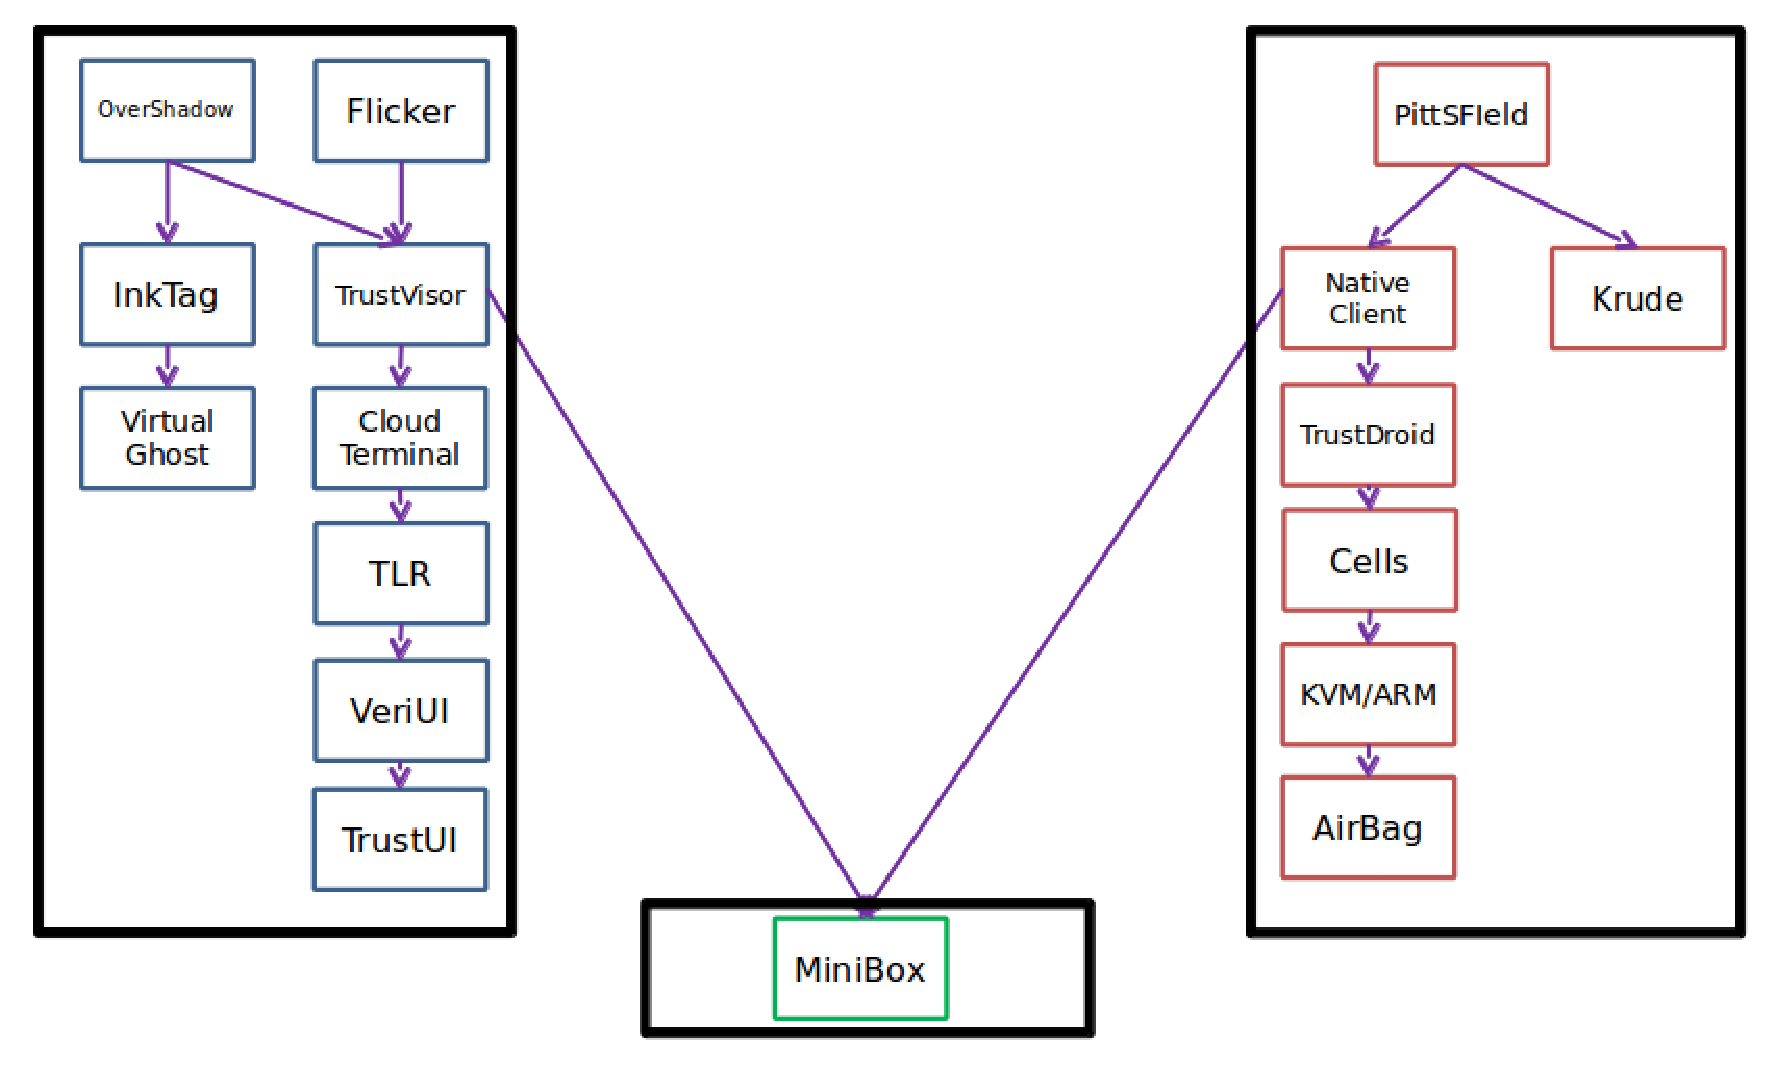
\includegraphics[width=\columnwidth]{figures/evolution.eps}
\caption{Evolution graph of prior works. The left branch includes prior works
when application is trusted but OS is malicious. The right branch includes prior
works when application is untrusted but OS is benign. MiniBox is the combination
of two branches.}
\label{fig:evolution}
\end{figure*}

In this talk, we discuss the evolution of the prior research works. We organize
previous works based on the problems classification and essential design
considerations when building solutions. The evolution graph of prior works on
the three problems is in Figure \ref{fig:evolution}. In section
\ref{sec:problem1}, we discuss the protection of secure application from the
untrusted operating system. Section \ref{sec:problem2} is about the isolation of
untrusted application from benign operating system. In section
\ref{sec:problem3}, we discuss MiniBox, the most up-to-date research work on
removing trust between application and the underpinning operating system.

\section{Secure App on Untrusted OS}
\label{sec:problem1}

\subsection{OS can be untrusted}

Although commodity operating systems are developed by extremely professional
software developers, the security provided by commodity operating systems is
often inadequate. Trusted OS components include not just the kernel but also
device drivers and system services that run with privilege (e.g., daemons that
run as root in Linux). Once such privileged code is compromised, an attacker
gains complete access to sensitive data on a system. The privileged operating
system kernel can read/write any code/data region of any user mode process. Both
privacy and integrity are imperiled by the hostile operating system.

Besides directly manipulating a secure application's state, the hostile
operating system kernel can also compromise the user mode application by Iago
attack \cite{Iago}. On commodity operating systems, the application and kernel
are conceptually peers and the system call API defines an RPC interface between
them. A carefully chosen sequence of integer return values to Linux system calls
can lead a supposedly protected process astray. The following sample code
demonstrates one Iago attack. It maps a 1024 byte region of memory via the mmap2
system call and then reads up to 1024 bytes into it from a file descriptor using
the read system call. Since the kernel is responsible for memory management,
instead of the address of the newly allocated memory region, returns an address
on the stack.  The stack will be overwritten with up to 1024 bytes of the
kernel's choice with the read system call. Therefore, a saved return address on
the stack may be overwritten and the program can be coerced into executing a
return-oriented program.

\begin{lstlisting}[language=C]
  p = mmap(NULL,1024,prot,flags,-1,0);
  read(fd,p,1024);
\end{lstlisting}

To protect the secure application from the malicious OS, a mechanism should be
used to isolate the secure application from the OS. In the meantime, the
isolated application should also be able to use the OS services. Ideally, the
Iago attack is prevented. In the following sections, we will discuss different
mechanism on secure application protection.

\begin{table*}[ht]
	\centering
	\begin{tabular}{|l|l|}
		\hline
		\textbf{Solution Category}      & \textbf{Research Papers} \\ \hline
		Trusted Hardware Based & Flicker \cite{Flicker}, TrustVisor \cite{TrustVisor} \\ \hline
		Hypervisor Based       & Overshadow \cite{Overshadow}, InkTag \cite{InkTag}, TrustVisor \cite{TrustVisor}, Cloud Terminal \cite{CloudTerminal}\\ \hline
		Instrumentation Based  & Virtual Ghost \cite{VirtualGhost}\\ \hline
		TrustZone Based        & TLR \cite{TLR}, VeriUI \cite{VeriUI}, TrustUI \cite{TrustUI}\\ \hline
	\end{tabular}
	\caption{Solution categorization on the protection of secure application
	(PAL) from the untrusted OS.}
	\label{my-label}
\end{table*}

\subsection{Trusted Hardware based}

Trusted Hardware allows the execution of pieces of application logic (PAL) in an
isolated environment. Flicker \cite{Flicker} leverages the hardware support for
Trusted Platform Module (TPM) and late launch recently introduced from AMD's
Secure Virtual Machine (SVM) technology. SVM chips are designed to allow the
late launch of the software (e.g. Virtual Machine Monitor or Security Kernel) at
an arbitrary time with the SKINIT instruction in CPU protection ring 0. As part
of the SKINIT instruction, the processor first causes the TPM to reset the
values of PCRs 17-23 to zero, and then transmits the contents of the PAL to the
TPM so that it can be measured and extended into PCR 17. Software cannot reset
PCR 17 without executing another SKINIT instruction. PALs can leverage TPM-based
sealed storage to maintain state across Flicker sessions. Therefore, the
sensitive task can be spitted into multiple sessions

However, Flicker's performance is not promising, especially for multi-session
PAL. At the beginning of each session, the TPM should decrypt sealed data from
persistent storage to recover the state of the previous session of this PAL. At
the end of this session, the TPM seals the data again and stores the data on
persistent storage. The frequent encryption/decryption undermines the
performance of Flicker. TrustVisor \cite{TrustVisor} improves the performance of
Flicker by simulating the TPM-based cryptography operations on a micro-TPM. The
micro-TPM is simulated by CPU chip. TrustVisor, which is a tiny hypervisor, is
booted with the late launch. It is responsible for the registration, invoke and
unregistration of all PALs.  TrustVisor isolates PAL from the untrusted
operating system with the nested page table (NPT). Hardware TPM attests the
integrity of the tiny hypervisor and the integrity of PAL is attested by the
software emulated micro-TPM. TrustVisor is the combination of both trusted
hardware and hypervisor based solutions. 

\subsection{Hypervisor based}

As we mentioned in last section, hypervisor can isolate the secure application
from the untrusted operating system. Overshadow \cite{Overshadow} utilizes a
binary translation based hypervisor with a mechanism called cloaking to prevent
the guest operating system from reading or tampering application code, data and
registers.  Cloaking is the mechanism to present an application context with a
cleartexted view of its pages, and the OS context with an encrypted view. At any
point in time, the page is mapped into only one shadow page table - either a
protected application shadow used by cloaked user-space processes, or the system
shadow used for all other accesses. Overshadow introduces a shim into the
address space of the cloaked application, which cooperates with the VMM to
mediate all interactions with the OS. The shim uses an explicit hypercall
interface for interacting with the VMM. System call transitions between
guest-user mode and guest-kernel mode are always trapped by a Binary Translating
VMM.

However, Overshadow has focused on simply isolating trusted code and data from
the OS, with minimal support for securely using OS features, that is, it is not
able to prevent Iago attack. It also doesn't support flexible access control and
crash consistency. InkTag proposes paraverification, a technique that simplifies
the hypervisor by forcing the untrusted OS to participate in its own
verification. InkTag requires the untrusted OS to provide information and
resources to both the hypervisor and application that allow them to efficiently
verify the operating system's actions. Verifying that the OS provides system
services correctly allows InkTag to avoid having to reason about the OS's
implementation of these services. Trusted application code executes in a high
assurance process, or HAP, which is isolated from the OS. Nearly all
application-level changes are contained in a small, 2000-line library
(libinktag) the use of which is largely encapsulated in the standard C library.

Cloud Terminal \cite{CloudTerminal} protects the secure application by running
the software on the remote server, instead of locally. In Cloud Terminal, the
only software running on the client, with which the user interacts, is a
lightweight secure thin terminal whose primary functionality is to render the
bitmap to be rendered sent by the remote server. Most application logic is in a
remote cloud rendering engine on the remote server. On the client side, the
secure thin terminal is isolated and protected by the hypervisor. The tiny
hypervisor helps supply a secure display and input path to remote software. The
secure thin terminal has a very small TCB (23 KLOC) and no dependence on the
untrusted OS, so it can be easily checked and remotely attested to.

\subsection{Instrumentation based}

Virtual Ghost protects application from a compromised or even hostile OS. It
leverages compiler instrumentation (with LLVM) create ghost memory that the
operating system cannot read or write. Virtual Ghost is based on the Secure
Virtual Architecture (SVA). In SVA, all kernel and module code must first go
through LLVM intermediate representation form (bitcode). The SVA VM translates
code from virtual instruction set to the native instruction set of the hardware.
SVA adds a set of instructions to LLVM called SVA-OS; these instructions replace
the hardware-specific operations used by an OS to communicate with hardware and
to do low-level state manipulation. During the translation from virtual
instruction to native instruction, load/store operations are instrumented so
that access to secure memory pages can be prevented from OS without unmapping or
encrypting secure pages. Virtual Ghost also enforces Control Flow Integrity
(CFI) on kernel code in order to ensure that the compiler instrumentation of
kernel code is not bypassed. Virtual Ghost outperforms InkTag.

\subsection{TrustZone based}

\begin{figure}[htb]
\centering
\includegraphics[width=\columnwidth]{figures/trustzone.eps}
\caption{Split CPU Mode with TrustZone Support}
\label{fig:trustzone}
\end{figure}

Considering the limited computing resources on smartphones, hypervisor and
instrumentation based solutions are not applicable to the smartphone. TrustZone
is utilized on smartphone to protect the secure application. TrustZone is a
hardware security technology incorporated into recent ARM processors. With
TrustZone, the processor can execute instructions in one of two possible
security modes, referred to as the normal world, where untrusted code executes,
and the secure world, where secure services run as in Figure
\ref{fig:trustzone}. These processor modes have independent memory address
spaces and different privileges. While code running in the normal world cannot
access the secure world address space, code running in the secure world can
access the normal world address space in certain conditions. Besides memory,
peripherals and interrupt are also world-sensitive. World switch is done via a
special instruction called the Secure Monitor Call (smc).

Trusted Language Runtime (TLR) \cite{TLR} is a system that protects the
confidentiality and integrity of .Net mobile application from OS security
breaches by separating and isolating the application's security-sensitive logic
from the rest of the application. TLR and security-sensitive code are in the
secure world of TrustZone. TLR is a small runtime engine that is capable of
interpreting .Net managed code inside a trusted secure environment. It is
carefully crafted by borrowing parts of the runtime engine design from the .NET
Micro Framework (NETMF) so that the TCB is significantly smaller than a
full-blown .NET framework and a full-featured OS. Security-sensitive code and
data are in a Trustbox which is an isolation runtime environment that protects
the integrity and confidentiality of code and data. The Trustlet specifies the
secure data and an interface that defines what data can cross the boundary
between the Trustbox and the untrusted world. With TLR, the developer should
manually split the application into sensitive and nonsensitive part.  A secure
application can package the code handling sensitive data into TrustLet and run
it in the TrustBox in the Secure World.

However, TLR does not support direct I/O within the Secure World. VeriUI
\cite{VeriUI} is able to securely handle user inputs (i.e., passwords) and
communication with remote servers. Smartphone applications often augment their
functionality by accessing user data mentioned by services such as Twitter and
Facebook. VeriUI is proposed to prevent phishing attacks by untrusted OS through
a secure and isolated environment for password input and transmission. An app
can invoke a web browser running in the secure environment of TrustZone to
retrieve an OAuth token after the user successfully authenticates. Even the
malicious OS cannot have access to the password data.  The secure kernel running
in secure environment can use its protected resources (i.e., a vendor-installed
public-key pair) to generate a signed attestation that includes a hash of the
Secure World's system software as well as information about the user's login
request.

As VeriUI runs a Linux in TrustZone secure world to provide the attested login
for users, it has a very large TCB. TrustUI \cite{TrustUI} takes a step further
by excluding drivers for user-interacting devices like touch screen from its
trusted computing base. TrustUI is a new trusted path design for mobile devices
that enables secure interaction between end users and services. It is based on
ARM's TrustZone technology and requires no trust of the commodity software
stack. TrustUI adopts a mechanism that logically splits a device driver into two
parts: a backend running in the normal world and a frontend running in the
secure world. The backend part is the unmodidied driver and its corresponding
wrapper in the normal world, while the frontend part works on top of it and
provides safe access to device for secure pages. The two parts communicate
through corresponding proxy modules running in both worlds which exchange data
through shared memory.



\section{Untrusted App on Benign OS}
\label{sec:problem2}

In this section, we discuss the protection of the operating system from an
untrusted application or a piece of untrusted code. In this paper, we call both
of untrusted application and untrusted code as untrusted module. The untrusted
module can be pieces of native code downloaded by a web browser, an application
uploaded and executed on the PaaS server, or an Android application downloaded
from an untrusted third part. Although the isolation of untrusted module can
prevent it from infecting the operating system, it is far from enough. There are
other challenges. First, the isolated code module wants to interact with the
operating system services via system calls. Second, the isolation (sandbox)
should not impact the performance of program execution. Third, a low
implementation overhead is expected, that is, the modification to compiler,
linker, application source code and operating system kernel source code should
be minimized. Last, since the smartphone has limited resources, the isolation
should be lightweight. 

In this paper, we categorize the prior works according to the granularity of
isolation. The granularity of isolation varies, including intro-process,
inter-process, inter-namespace and inter-VM. 

\begin{table*}[ht]
	\centering
	\begin{tabular}{|l|l|}
		\hline
		\textbf{Solution Category}      & \textbf{Research Papers} \\ \hline
		Inter-VM Based         & KVM/ARM \cite{KVM/ARM} \\ \hline
		Intra-Process Based    & SFI \cite{SFI}, PittSFIeld \cite{PittSFIeld}, Native Client \cite{NaCl} \\ \hline
		Inter-Process Based    & Native Client \cite{NaCl}, Krude \etal \cite{Krude} \\ \hline
		Inter-Namespace Based  & TrustDroid \cite{TrustDroid}, Cells \cite{Cells}, AirBag \cite{AirBag} \\ \hline	
	\end{tabular}
	\caption{Solution categorization on the protection of OS from the untrusted
	application.}
	\label{my-label}
\end{table*}

\subsection{Inter-VM based}
\label{sec:problem2:inter-vm}

The naive approach is to isolate each untrusted module into its correpsonding
VM. There are a variety of virtual machine monitors, including Xen, KVM, Qemu,
and VMWare.  Recently, the hardware virtualization extension has been added into
the ARM and the ARM based KVM \cite{KVM/ARM} is integrated into the Linux kernel
since Linux 3.9. Since this approach is clear and self-explained, we will not
discuss it in detail in this paper.

\subsection{Intra-Process based}
\label{sec:problem2:intra-process}

Intra-Process protection is to isolate the untrusted module from the other
memory regions in the same address space. SFI \cite{SFI} is proposed to sandbox
the untrusted module by rewriting the untrusted code at the instruction level,
that is, to instrument store/load and control flow instructions. However, it
only works for RISC architectures. PittSFIeld \cite{PittSFIeld} presents
sandboxing technique that can be applied to CISC architecture e.g. IA-32, and
whose application can be checked at load-time to minimize the TCB.  Unlike RISC
architectures, whose instructions have the same length, the x86 has
variable-length instructions that might start at any byte. To avoid this
problem, PittSFIeld divides memory into segments whose size and location is
16-byte aligned.  New instructions are instrumented before store/load and
control flow instructions to check that the sandboxed module cannot read/write
data outside sandbox and transfer to illegal control flow target outside
sandbox.

A weakness of PittSFIeld is it cannot effectively mediate the access from
untrusted module to operating system services. Besides isolating the untrusted
module, Native Client \cite{NaCl} also allows the module to interact
with services, such as file I/O and local database access, by the combination of
intra-process and inter-process approaches.  An Intra-Process based sandbox is
used to isolate the untrusted module from the runtime service, which resides in
the same address space as the sandboxed untrusted module. Runtime service
mediates the communication between the untrusted module and other processes
including web browser and other services. This is similar to the Inter-Process
based solution in the next section.

\subsection{Inter-Process based}
\label{sec:problem2:inter-process}

Krude \etal \cite{Krude} is an inter-process based isolation approach to sandbox
the untrusted module. It is specifically designed for PaaS architectures, where
code execution needs to be isolated to protect tenants from unauthorized access
to their data by other tenants and to protect the host system from any type of
intrusion by other tenants. The untrusted module is uploaded to the PaaS server
and it is isolated in a new process. Krude \etal uses the process barrier and
the seccomp filter mechanism to restrict access to memory and to the system call
interface. Almost all system calls are blocked for the isolated process. Besides
memory allocation and deallocation, the isolate can communicate with OS by
sending to request to a supervisor process via pipe, which is the IPC mechanism
on Linux. The supervisor process will process the request and send the response
back to the isolated process also via pipe.

\subsection{Inter-Namespace based}
\label{sec:problem2:inter-namespace}

The Inter-Namespace based approach is primary proposed for smartphone running
Android. Nowadays, smartphones are ubiquitous. Many use the smartphone both for
working and personal needs. However, the personal applications downloaded from
the untrusted website can compromise the application issued by the trusted
enterprise. Therefore, many users carry multiple phones to accommodate work,
personal and geographic mobility need. Cells proposes a smartphone
virtualization solution so that multiple virtual smartphones can run
simultaneously on the same physical smartphone in an isolated, secure manner.
Unlike the virtualization techniques mentioned in section
\ref{sec:problem2:inter-vm}, Cells leverages a lightweight OS-level
virtualization by the utilization of namespace. Linux namespace is being used by
OpenVZ and LXC. A set of processes can be grouped into the same namespace. Each
Linux namespace has PID namespace isolation, network namespace isolation, UTS
namespace isolation, mount namespace islation and IPC namespace isolation.

Cells observes that smartphones display only a single application at a time, and
introduces a usage model which has one foreground Virtual Phone (VP) that is
displayed and multiple background VPs that are not displayed at any given time.
The foreground VP is always given direct access to hardware devices while the
back ground VPs are given shared access to hardware devices when the foreground
VP does not require exclusive access. Cells provides novel kernel-level and
user-level device namespace mechanisms to efficiently multiplex hardware devices
across multiple VPs. Therefore, untrusted application inside personal VP
(namespace) will not be able to compromise the trusted application inside
enterprise VP. 

While Cells aims to embrace the emerging Bring-Your-Own-Device (BYOD) paradigm,
each VP is treated equally and the isolation is achieved at the coarse-grained
VP boundary. Unlike Cells, AirBag \cite{AirBag}'s objective is to boost the
smartphone's defense capability against the malware infection by isolating the
untrusted application in the AirBag environment. By dynamically creating an
isolated runtime environment with its own dedicated namespace and virtualized
system resources, AirBag is able to protect the OS from the malicious untrusted
applications, e.g., an Android game repacked with the malware. AirBag creates
and decouples an Application Isolation Runtime (AIR) from the native Android
runtime, which contains Java \& Native Libraries, Application framework (e.g.,
SurfaceFlinger service) and Dalvik virtual machine.  AIR does not need to be
trusted as it might be potentially compromised by untrusted application. AirBag
multiplexes hardware resources between the AIR and native runtime by either
creating a second resource (e.g., memory buffer) or creating a proxy between
runtimes and hardware to mediate access from different runtimes.




\section{Two-Way Protection}
\label{sec:problem3}

We discussed the protection of secure application from untrusted OS (e.g.,
TrustVisor \cite{TrustVisor}) in section \ref{sec:problem1} and the protection
of benign OS from untrusted application (e.g., Native Client \cite{NaCl}) in
section \ref{sec:problem2}. In this section, we discuss the removing of trust
between the application and operating system. Within my knowledge, currently,
MiniBox \cite{MiniBox} is the first and the only attempt toward a practical
two-way sandbox for x86 native applications by combining TrustVisor and
Native Client.

Platform-as-a-Service (PaaS) is one of the most widely commercialized forms of
cloud computing. According to Google, in 2012, there were 1M active
applications running on Google App Engine \cite{engine}, where untrusted
applications are sent by customers. Therefore, it is critical to protect the
cloud platform from the untrusted applications. Besides cloud provider such as
Google, security on PaaS is also a concern for cloud customers. People should
rethink the security model of PaaS cloud computing because a two-way sandbox is
desired.

Although it seems promising to combine a one-way sandbox (e.g., TrustVisor) and
a two-way memory isolation mechanism (e.g., Native Client) to establish two-way
protection, there are many challenges. First, the deliberate system design is
required. Second, the interface between software modules for OS protection and
the application should be minimized and secure. Finally, the design of
TrustVisor doesn't support Iago attack prevention. The final system design
should be able to protect application against Iago attack.

\begin{figure}[htb]
\centering
\includegraphics[width=\columnwidth]{figures/minibox.eps}
\caption{MiniBox Architecture}
\label{fig:minibox}
\end{figure}

MiniBox \cite{MiniBox} combines the one-way sandbox for x86 native code and
hypervisor-based two-way memory isolation. As in figure \ref{fig:minibox}, the
sandbox is split into service runtime modules and OS protection modules. The
service runtime is included in the isolated memory space with the application
together to support application execution. The original disassembly based
sandbox is not required anymore because the hypervisor not only isolates the
application from OS, but also isolates the OS from the application. To prevent
Iago attacks, the system calls are divided into sensitive calls and
non-sensitive calls. All sensitive calls are handled directly by a LibOS
\cite{LibOS}, which the application trusts, residing at the Mutually Isolated
Execution Environment (MIEE).  Non-sensitive calls will be forwarded to the
Regular Environment (RE). The OS in RE handles the non-sensitive calls mediated
by the OS protection module in RE. 

\section{Discussion}
\label{sec:discussion}

\section{Future Work}
\label{sec:future}

Most prior works on PC are based on x86 architecture, e.g., Intel and AMD. x86
based servers are not energy efficient. To handle hundreds of millions of users
and their associated transactions, companies such as Amazon, Facebook, and
Google run immense data centers with until-recently unimaginable computation and
storage capacities. As online services become pervasive, projections indicate
that electricity consumed in global data centers worldwide in 2010 is more than
200B KWh, between 1.1\% and 1.5\% of worldwide electricity use. Three years ago,
Google announced that their facilities have a continuous electricity usage
equivalent to powering 200,000 homes.Therefore, it is promising to replace x86
with ARM architecture to build the next generation of servers in the cloud.
There are already many ARM development boards published, such as Raspberry Pi,
BeagleBone and Cubitruck. 

In the future, we want to explore the security problems on ARM architecture.
Although prior works such as TLR \cite{TLR}, VeriUI \cite{VeriUI} and TrustUI
\cite{TrustUI} use security features of ARM, they are designed especially for
smartphones. We propose the first solution to execute the secure PAL on ARM
architecture both on a single server or in the cloud environment. Virtualization
can effective achieve the mutually memory isolation between application and OS.
However, currently the hardware virtualization extension is not supported by all
ARM CPUs.

\begin{figure}[htb]
\centering
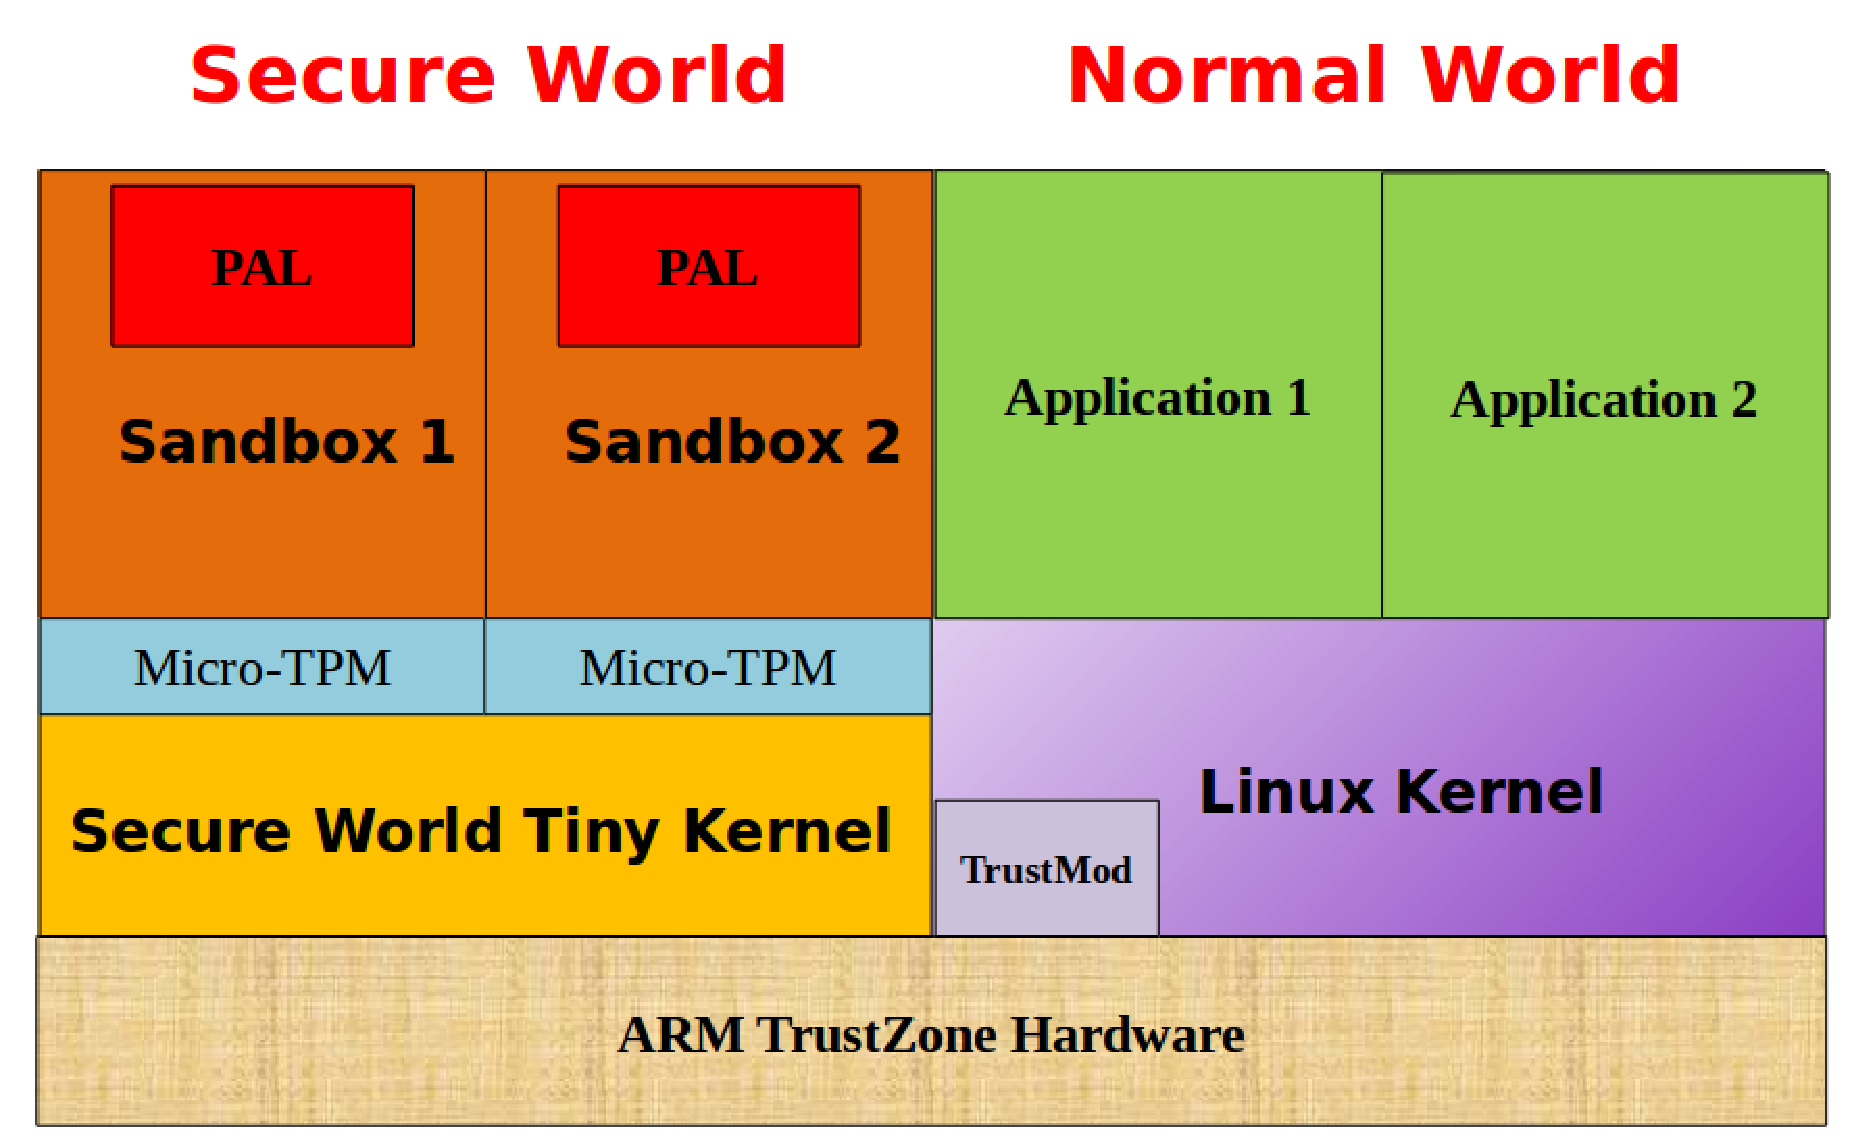
\includegraphics[width=\columnwidth]{figures/future.eps}
\caption{Secure execution of PAL on ARM}
\label{fig:future}
\end{figure}

Our proposal, as in Figure \ref{future}, leverages the TrustZone, which is supported by most ARM CPUs, to
isolate the secure PAL in the secure world. The regular OS is running in the
normal world. The secure PAL is executed in the secure world. Unlikne
virtualization which can create more than one isolated environment, there is
only one secure world with TrustZone. To prevent the secure PAL of one
application from compromising the PAL of another, all PALs are sandboxed in the
secure world. We will use TrustZone to emulate the secure boot, late launch and
TPM operations. As ARM boards usually have limited resources, , the secure world
tiny kernel will not be loaded into memory unless the execution of PAL is
registered and triggered. To prevent Iago attack, we divide the system calls
into sensitive calls and non-sensitive calls. All sensitive calls, which can be
used by malicious OS to mount the Iago attack, will be handled directly by the
tiny kernel in secure world. Non-sensitive calls will be redirected to the
untrusted OS in normal world. As the tiny kernel is only responsible for
supporting the Micro-TPM, memory management and handling sensitive system call,
the TCB is small.  

\section{Conclusion}
\label{sec:conclusion}

The protection of secure application from malicious OS and the sandbox of
untrusted application from benign OS on the PC are two relatively mature
research topics that have made substantial advances over the last decade.
However, how to remove the trust between the application and OS on both PC and
smartphone is still not fully explored.  Prior works also have limitations,
e.g., the granularity of protection and performance overhead. In this paper, we
discuss the evolution of prior works on the three problems.  More future works
are expected especially for smartphone and ARM-based server/cloud. Future cloud
computing framework should balance security, performance, cost and mobility.


\bibliographystyle{plain}
\bibliography{refs}

\end{document}
